\documentclass[12pt,a4paper]{article}
\usepackage{amsmath}
\usepackage{amsfonts}
\usepackage{amssymb}
\usepackage{graphicx}
\begin{document}

\section{splines caclulations}
Splines data points are calculated at fixed energies. The energy points are uniformly distributed in logarithmic range.
The number of points and logarithmic limits are defined in \textit{constants.h}.
The number of points is \textit{max\_datapoints}, log limits are \textit{logEmin} and \textit{logEmax}.


The energy points are stored in \textit{EnergyTable} class and precalculated values are stored in \textit{energy\_table} variable.
the double array can be accessed as energy\_table.values.

The integration is done using GSL numerical integration library.

\subsection{range spline precision}
The range spline precision is checked via calculating dE/dx from inverse derivative of range spline and compared to directly calculated dE/dx.

\begin{figure}[h]
	\centering
    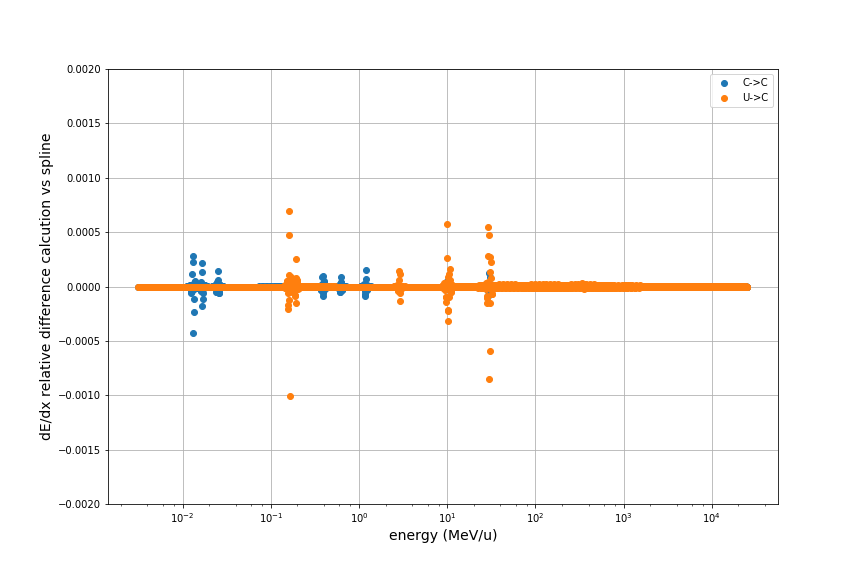
\includegraphics[width=6.5cm]{plots/dedx_difs_n500.png}
   	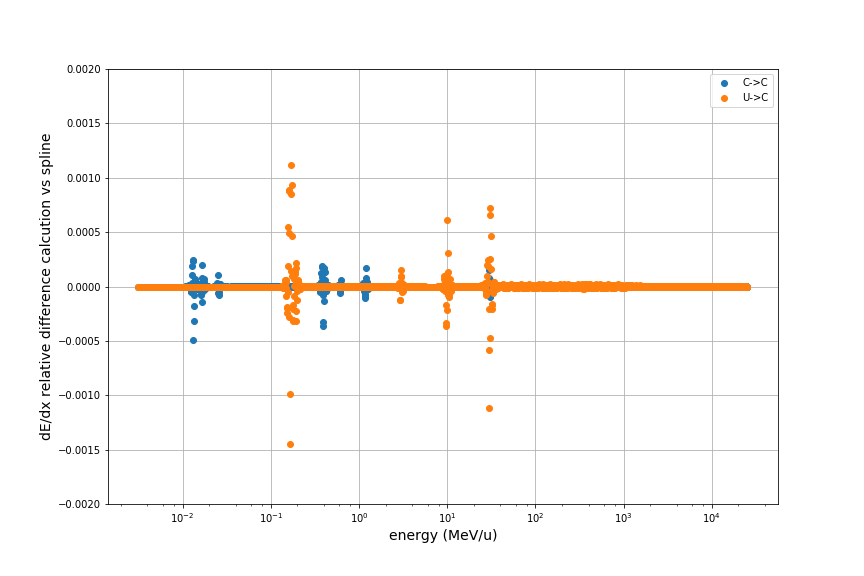
\includegraphics[width=6.5cm]{plots/dedx_difs_n400.png}
   	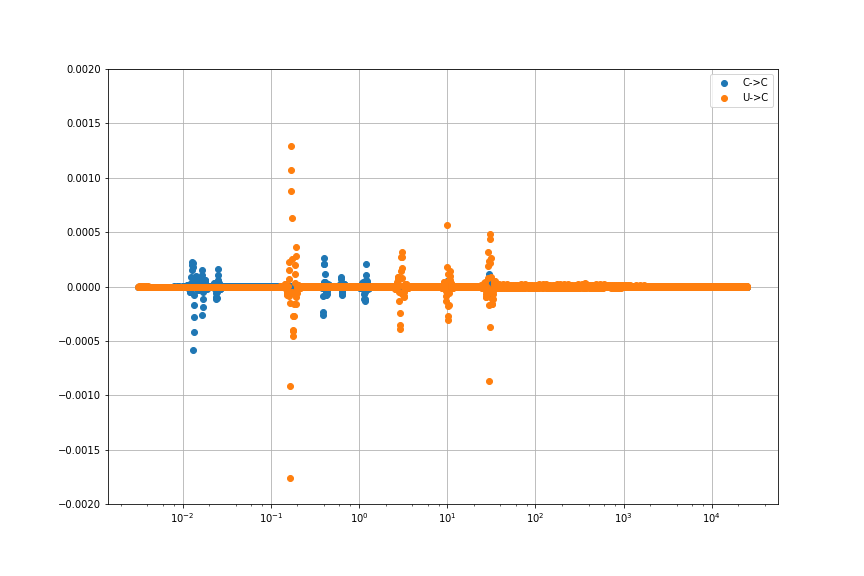
\includegraphics[width=6.5cm]{plots/dedx_difs_n300.png}
   	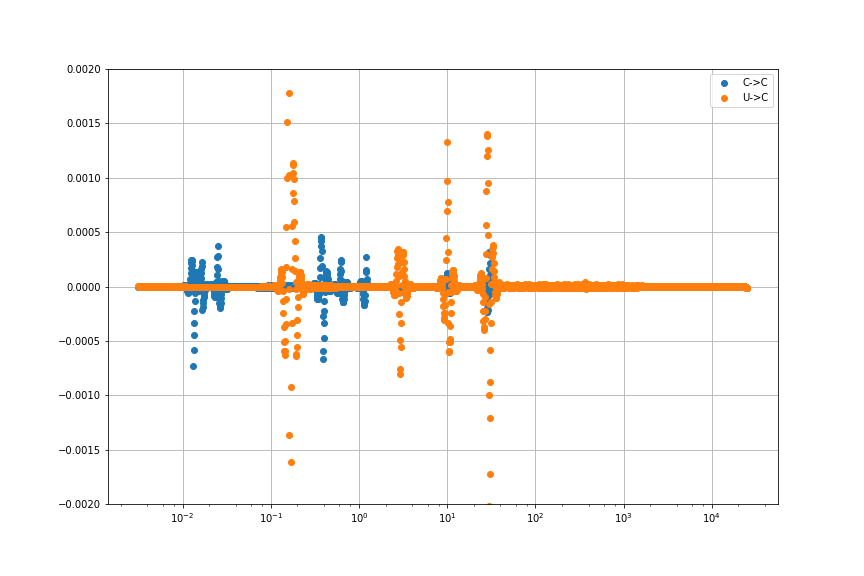
\includegraphics[width=6.5cm]{plots/dedx_difs_n200.png}
	\caption{Relative difference of dE/dx calculated directly and from range spline, number of range spline datapoints = 500(top left), 400(top right), 300(bottom left), 200(bottom right)}
\end{figure}	


\section{Lindhard-Soerensen}
The Lindhard-Soerensen (LS) corrections to energy loss and energy loss straggling can be calculated directly or from precalculated values, which is useful when performance is needed. The precalculated LS coefficients are calculated at predefined log distributed energies. Below and above the energy limits the functions returns the value at minimal or maximal precalculated value. The take into account the different masses the Ls coefficients are precalculated for 2 different masses and final coefficients are estimated using a linear interpolation between the two calculations.


The calculated LS coefficients are plotted in Fig. \ref{ls}. 
For the comparison and check of precalculated LS coefficients the LS coefficients and relative difference to directly calculated coefficients for different masses and charges are plotted in Figures \ref{ls_prec} amd \ref{lsX_prec}.

\begin{figure}
\centering
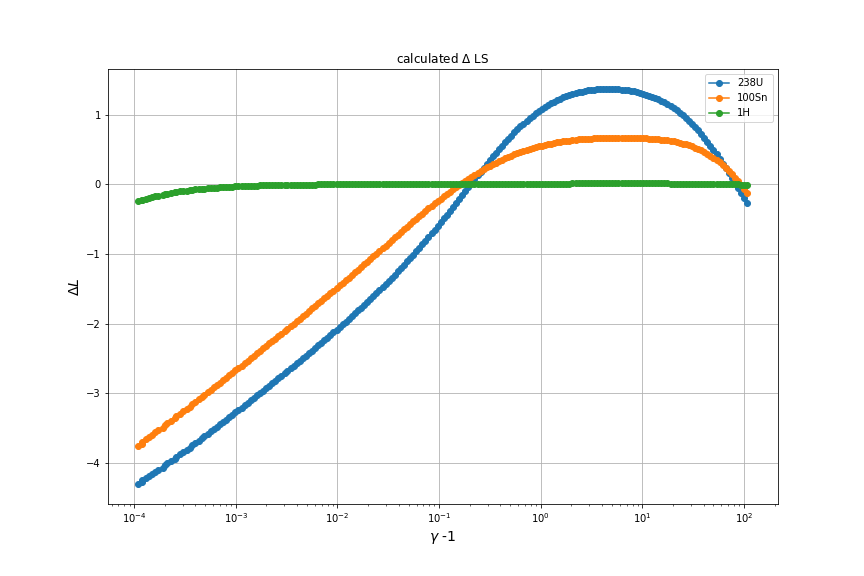
\includegraphics[width=6.5cm]{plots/ls.png}
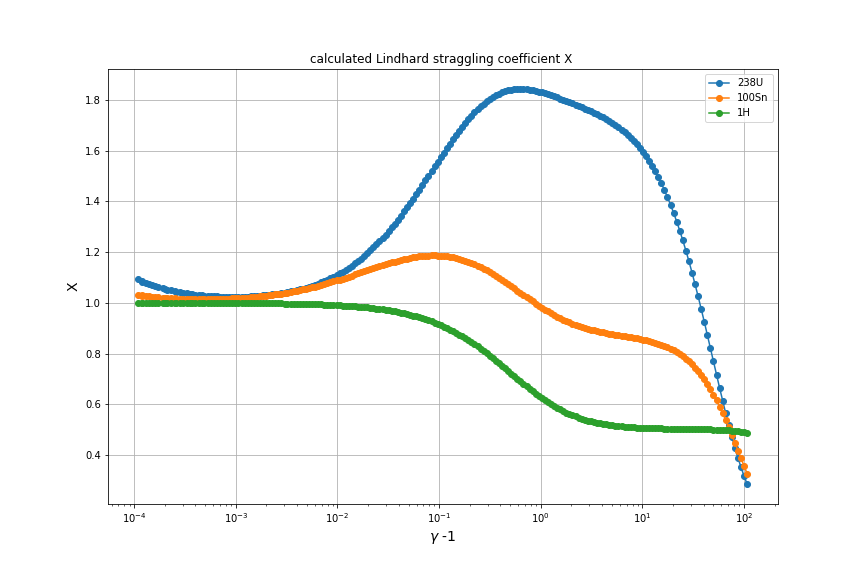
\includegraphics[width=6.5cm]{plots/lsX.png}
\caption{LS corrections for energy loss and energy loss straggling for different energies and projectile}
\label{ls}
\end{figure}

\begin{figure}
\centering
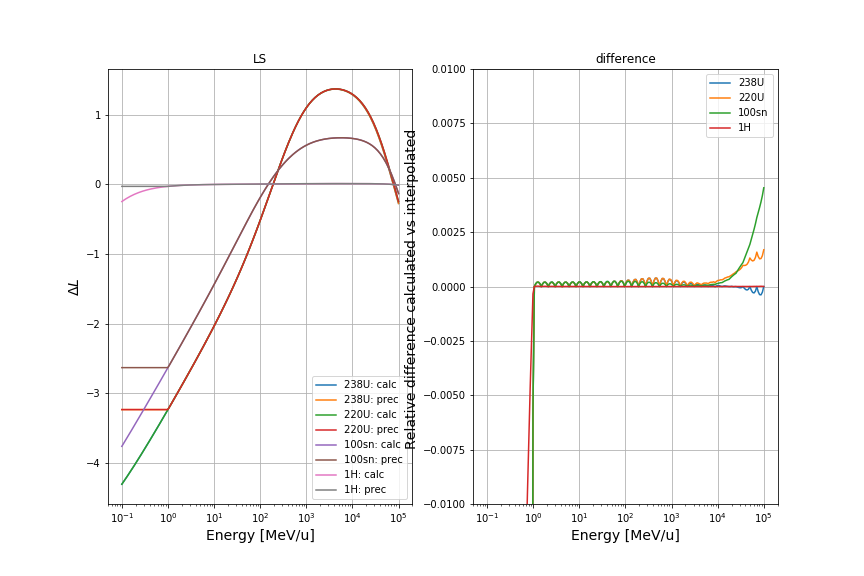
\includegraphics[width=12cm]{plots/ls_precision.png}
\caption{LS corrections for energy loss directly calculated and calculated from the tabulated values for different Z and A. On the right the relative differences are plotted. The lowest energy for precalculation was set to 1 MeV/u.}
\label{ls_prec}
\end{figure}

\begin{figure}
\centering
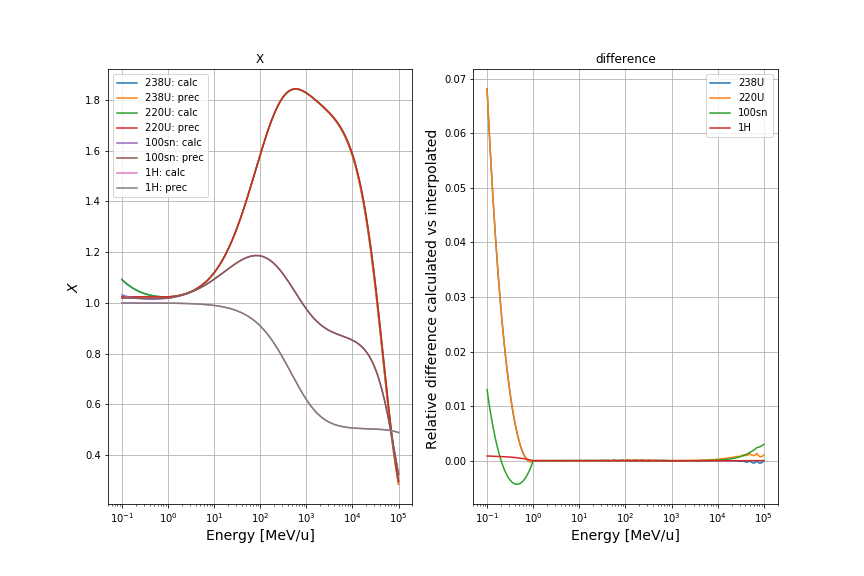
\includegraphics[width=12cm]{plots/lsX_precision.png}
\caption{LS corrections for energy loss directly calculated and calculated from the tabulated values for different Z and A. On the right the relative differences are plotted. The lowest energy for precalculation was set to 1 MeV/u.}
\label{lsX_prec}
\end{figure}




\section{Benchmarks}
\subsection{Thin Target Approximation}
test: projectile: 238U@700MeV/u - 30GeV/u, material: C(1mg/cm2), 30000 calculation in loop.
reults: with thin target pproximation: 2.4s, without: 2.4s
	
\end{document}